\begin{titlepage}

  \newcommand{\HRule}{\rule{\linewidth}{0.5mm}} % Defines a new command for the horizontal lines, change thickness here
  
  \center % Center everything on the page
   
  %----------------------------------------------------------------------------------------
  %	HEADING SECTIONS
  %----------------------------------------------------------------------------------------
  
  %\textsc{\LARGE University Name}\\[1.5cm] % Name of your university/college
  %\textsc{\Large Major Heading}\\[0.5cm] % Major heading such as course name
  %\textsc{\large Minor Heading}\\[0.5cm] % Minor heading such as course title
  
  %----------------------------------------------------------------------------------------
  %	TITLE SECTION
  %----------------------------------------------------------------------------------------
  
  \HRule \\[0.4cm]
  { \huge \bfseries Project : \textsc Make 360 degres Objects Renders  }\\[0.4cm] % Title of your document
  \HRule \\[0.4cm]

  %----------------------------------------------------------------------------------------
  %	AUTHOR SECTION
  %----------------------------------------------------------------------------------------
  
  %\begin{minipage}{0.4\textwidth}
  %\begin{flushleft} \large
  %\emph{Author:}\\
  %John \textsc{Smith} % Your name
  %\end{flushleft}
  %\end{minipage}
  %~
  %\begin{minipage}{0.4\textwidth}
  %\begin{flushright} \large
  %\emph{Supervisor:} \\
  %Dr. James \textsc{Smith} % Supervisor's Name
  %\end{flushright}
  %\end{minipage}\\[2cm]
  
  % If you don't want a supervisor, uncomment the two lines below and remove the section above
  \Large
  Students : Fréddéric \textsc{JENN ALET}\\ % Your name
  \Large
   Cyprien  \textsc{QUIVET}\\ % Your name
   \Large
   Class  \textsc{ Master SME}\\ % Your name
  

  
  \begin{figure}[b]
    \centering
    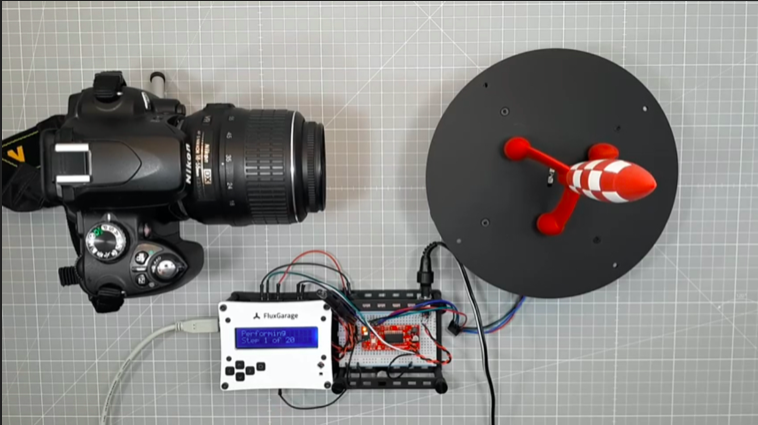
\includegraphics[scale=0.4]{img/presentation.png}\\% Include a department/university logo - this will require the graphicx package
    \label{fig:LogoTachyssema}
  \end{figure}
  %{%\Large  2020, April}\\[2cm] % Date, change the \today to a set date if you want to be precise

  
   
  %----------------------------------------------------------------------------------------
  
  \end{titlepage}